\chapter{Metodologia}

\section{Introdução à Metodologia}

A escolha metodológica de uma pesquisa define o caminho pelo qual as questões de estudo serão abordadas e os objetivos alcançados. No contexto deste estudo, a abordagem quantitativa foi selecionada devido à sua capacidade de fornecer resultados mensuráveis e replicáveis, importantes para a avaliação do desempenho dos algoritmos de aprendizado de máquina. Conforme destacado por \cite{Creswell2014}, a metodologia quantitativa permite uma investigação sistemática das propriedades e fenômenos quantificáveis, facilitando a comparação e a generalização dos resultados. Este estudo emprega uma metodologia quantitativa para explorar a eficácia dos algoritmos de classificação de texto em um conjunto de dados específico, buscando contribuições significativas para o campo do processamento de linguagem natural e aprendizado de máquina. A seleção desta abordagem está alinhada com os objetivos de pesquisa, que visam quantificar o desempenho dos modelos em tarefas de classificação de descrições de produtos em português, utilizando para isso o dataset RETAILPRODUCTDESCRITION-PTBR, especialmente preparado e anotado para este fim.

\section{Design da Pesquisa}

O design desta pesquisa adota uma abordagem quantitativa, estruturada para investigar o impacto de diferentes algoritmos de aprendizado de máquina na classificação de textos em português. Seguindo as recomendações de \cite{Yin2018}, que enfatiza a importância de um design de pesquisa claramente definido para estudos quantitativos, este estudo utiliza um design experimental para comparar o desempenho de vários algoritmos. Yin sugere que tal abordagem estabelece uma relação causal e permite compreender o efeito das variáveis independentes nas dependentes dentro de contextos controlados. O experimento é estruturado em fases distintas, incluindo a seleção de dados, pré-processamento, treinamento de modelos, e avaliação, visando um entendimento dos mecanismos que influenciam a eficácia da classificação de texto. Este design é particularmente adequado para a pesquisa em processamento de linguagem natural (PLN), permitindo análises detalhadas e replicáveis dos modelos computacionais em tarefas de classificação.

\section{Linguagem de Programação e Bibliotecas}

Para este trabalho, foi utilizada a Linguagem Python \cite{10.5555/1593511} e a biblioteca scikit-learn \cite{pedregosa2011scikit}.  A seleção da linguagem de programação Python e da biblioteca scikit-learn para a realização deste estudo foi baseada em múltiplas considerações técnicas e práticas, fundamentadas nas vantagens que ambas oferecem para projetos de aprendizado de máquina e processamento de linguagem natural.

\subsection{Vantagens da Linguagem Python}
\begin{itemize}
    \item \textbf{Rica Biblioteca de Pacotes:} Python é apreciada por seu vasto ecossistema de bibliotecas e frameworks, como NumPy, pandas e Matplotlib, facilitando a manipulação de dados, a análise estatística e a visualização.
    \item \textbf{Comunidade Ativa:} A extensa comunidade de usuários e desenvolvedores de Python proporciona um rico ambiente de recursos educacionais, documentação extensiva e suporte técnico.
    \item \textbf{Interoperabilidade:} Python oferece integração fácil com outras linguagens e tecnologias, permitindo a utilização de bibliotecas de alto desempenho escritas em C e C++.
\end{itemize}

\subsection{Vantagens da Biblioteca scikit-learn}
\begin{itemize}
    \item \textbf{Ampla Coleção de Algoritmos:} scikit-learn fornece uma extensa gama de algoritmos de aprendizado supervisionado e não supervisionado, pré-processamento de dados, seleção de modelos e avaliação, todos acessíveis por meio de uma interface consistente e bem documentada.
    \item \textbf{Documentação e Tutoriais:} A biblioteca é acompanhada por documentação abrangente e tutoriais detalhados que facilitam o aprendizado e a aplicação prática de métodos.
    \item \textbf{Desempenho e Eficiência:} scikit-learn é otimizado para performance, com vários de seus componentes internos implementados em Cython para melhorar a eficiência.
\end{itemize}

\section{Procedimento Experimental}

O procedimento experimental adotado neste estudo é delineado em duas fases principais, cada uma focada em aspectos distintos da modelagem para classificação de texto. Essas fases são visualmente representadas na Figura \ref{fig:workpipeline}.  Nas seções seguintes são descritas em mais detalhes cada item.

\begin{figure}[H]
    \centering
    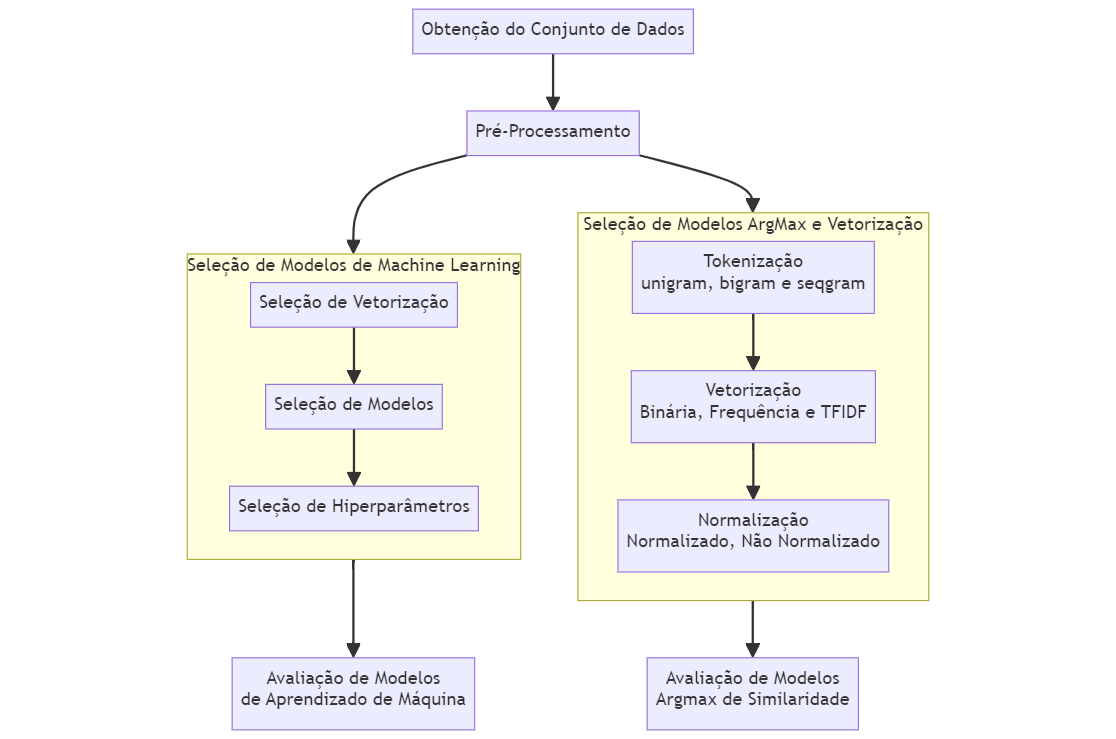
\includegraphics[width=0.8\textwidth]{images/fluxo.png}
    \caption{Fluxo de Trabalho.}
    \label{fig:workpipeline}
\end{figure}

\subsection{Conjunto de Dados}

O conjunto de dados foi obtido em \cite{dataset_2022}. Este conjunto de dados abrange descrições de produtos e suas respectivas categorias, coletadas dos dezoito maiores varejistas no Brasil, baseando-se na classificação da ABRAS do ano de 2020. Os itens selecionados representaram noventa e cinco por cento das vendas do ano de 2020 destes varejistas, representando os produtos mais vendidos das maiores redes varejistas do Brasil.

\subsubsection{Características Gerais}
O dataset é composto por 250.365 entradas e 7 colunas, detalhando descrições de produtos e informações taxonômicas. Os campos incluem \texttt{nm\_item}, \texttt{segmento}, \texttt{subsegmento}, \texttt{categoria}, \texttt{subcategoria}, \texttt{id\_product}, e \texttt{nm\_product}, todos categorizados como strings, exceto \texttt{id\_product} que é do tipo numérico. O número de valores únicos por coluna varia, indicando a diversidade dos produtos e sua classificação. Não existem registros nulos no dataset.

A tabela a seguir apresenta uma visão geral da estrutura hierárquica do conjunto de dados, destacando a organização e a especificidade com que os produtos são catalogados:

\begin{table}[h]
\centering
\begin{tabular}{ll}
\hline
\textbf{Nível de Classificação} & \textbf{Quantidade} \\
\hline
Segmentos              & 6          \\
Subsegmentos           & 20         \\
Categorias             & 70         \\
Subcategorias          & 169        \\
Categoria de Menor Nível & 795      \\
Descrições             & 250.365    \\
\hline
\end{tabular}
\caption{Visão geral da estrutura hierárquica do conjunto de dados.}
\label{table:estrutura_hierarquica}
\end{table}

\subsubsection{Detalhamento dos Campos e Hierarquia}

Para cada campo do conjunto de dados, é apresentado uma descrição a seguir:
\begin{itemize}
    \item \textbf{Nome do Item (\texttt{nm\_item})}: Este campo contém descrições dos produtos.
    \item \textbf{Segmento}: Funciona como uma classificação de nível superior, agrupando os produtos em categorias amplas. Com apenas seis categorias distintas, destaca uma divisão geral dos produtos.
    \item \textbf{Subsegmento}: Fornece uma subdivisão dos segmentos, oferecendo 20 categorias distintas para uma diferenciação mais detalhada entre os produtos.
    \item \textbf{Categoria}: Apresenta uma camada de classificação sob os subsegmentos com 70 categorias únicas.
    \item \textbf{Subcategoria}: Representa o quarto nível de classificação, com 169 subcategorias distintas.
    \item \textbf{Categoria de Nível Mais Baixo (\texttt{id\_product})}: Um código único atribuído a cada categoria de nível mais baixo, com 797 identificadores distintos, representa a menor granularidade hierárquica.
    \item \textbf{Descrição da Categoria de Nível Mais Baixo(\texttt{nm\_product})}: A descrição da categoria de menor granularidade hierárquica.
\end{itemize}

A estrutura hierárquica pode ser resumida na Figura \ref{fig:hierarquia}.
\begin{figure}[H]
    \centering
    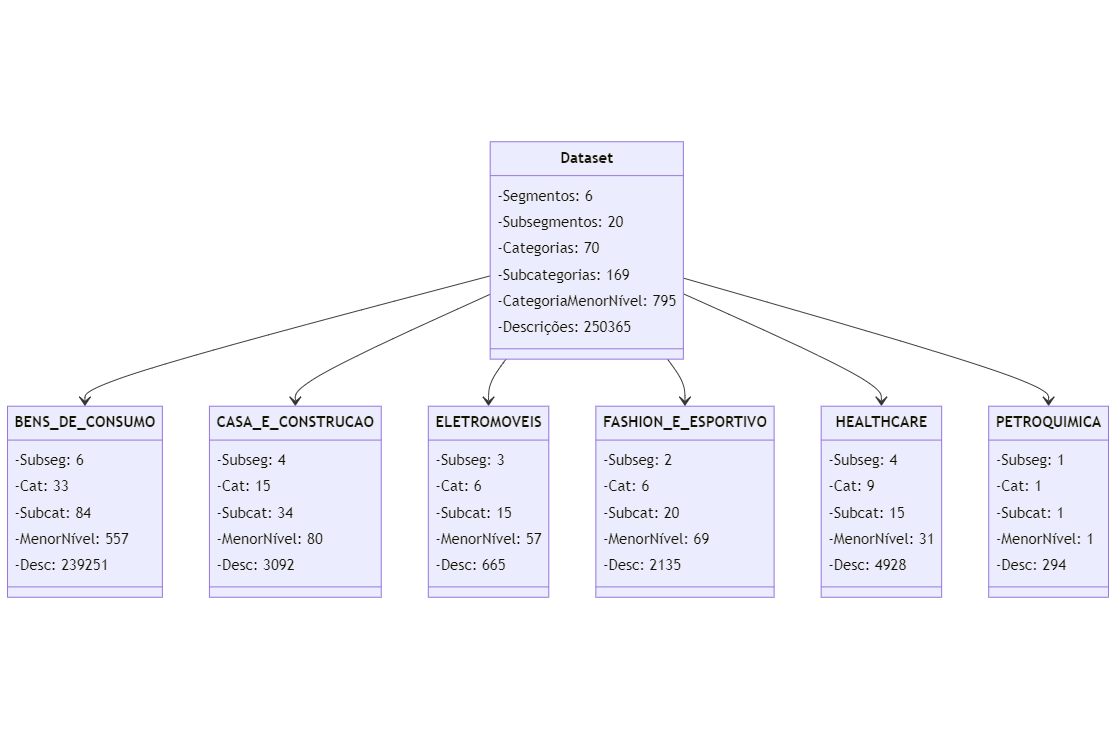
\includegraphics[width=0.8\textwidth]{images/hierarquia.png}
    \caption{Hierarquias}
    \label{fig:hierarquia e quantidade de elementos distintos e descrições em cada segmento}
\end{figure}


\subsubsection{Análise Exploratória de Dados (EDA)}

A Análise Exploratória de Dados é necessária para entender as características do conjunto de dados, permitindo a identificação de padrões, anomalias, e distribuições. As análises concentram-se em descrever características das descrições de produtos e a distribuição de rótulos pelas categorias de menor nível.

Inicia-se a análise pela distribuição das descrições pelas categorias utilizando a curva acumulada, figura \ref{fig:histdistclasses}.  A análise mostra que 70\% dos dados estão concentrados em 80 categorias de menor nível, indicando uma distribuição desigual. Este padrão ressalta a importância de algumas categorias no contexto dos varejistas.
\begin{figure}[H]
    \centering
    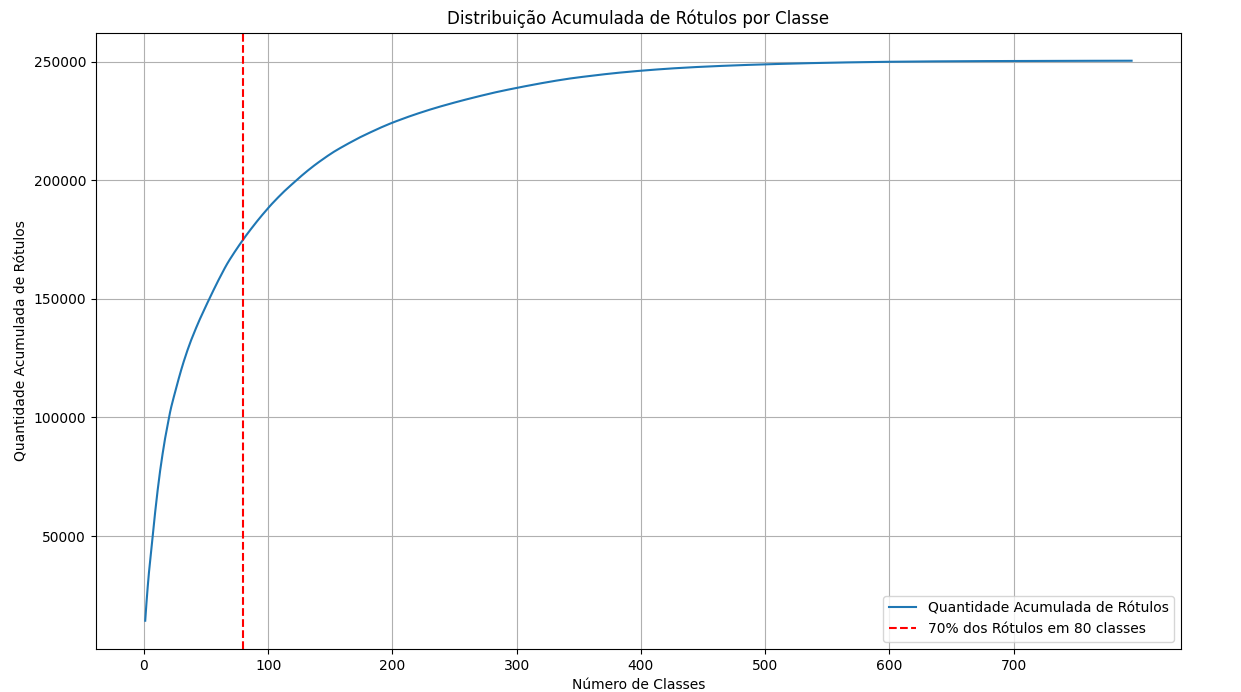
\includegraphics[width=0.8\textwidth]{images/histdistclasses.png}
    \caption{Distribuição das categorias de menor nível em escala logarítmica.}
    \label{fig:histdistclasses}
\end{figure}

Categorias como "BISCOITO" e "IOGURTE" lideram em quantidade de itens, refletindo as tendências de consumo. A Figura , Figura \ref{fig:grafico_barras_top10} exibe as 10 categorias com a maior quantidade de itens classificados.  Esta concentração denota o desbalanceamento e a dificuldade que se tem em tarefas de classificação.

 \begin{figure}[H]
    \centering
    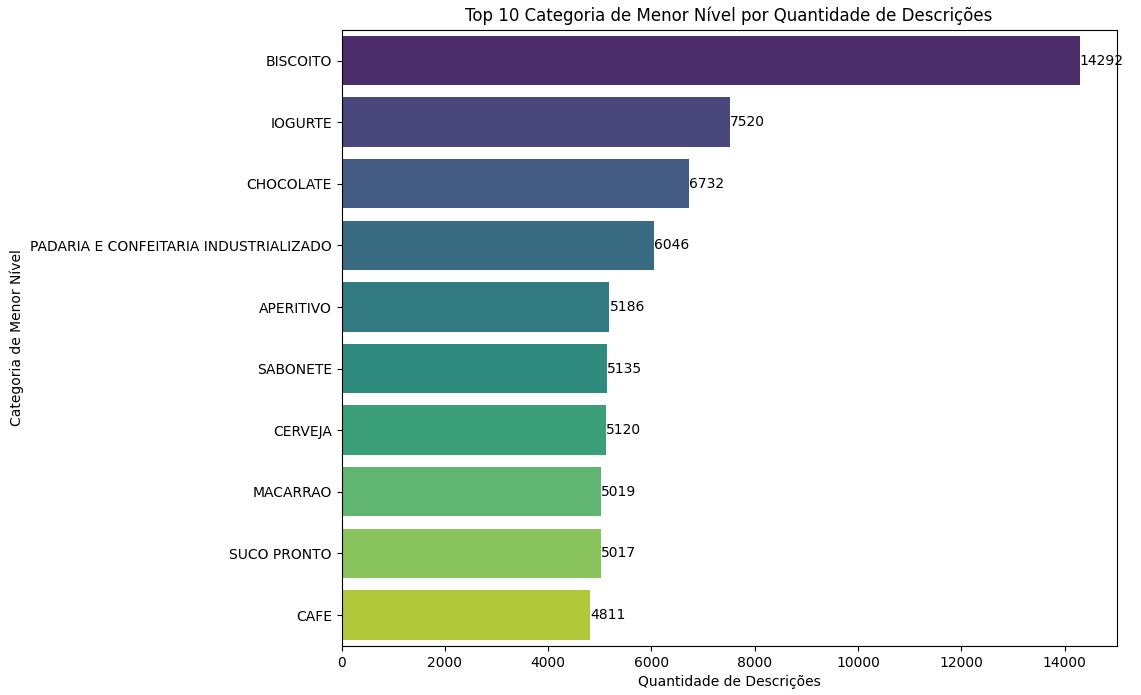
\includegraphics[width=0.8\textwidth]{images/grafico_barras_top10.png}
    \caption{Top 10 categorias de produtos com o maior número de rótulos.}
    \label{fig:grafico_barras_top10}
\end{figure}
\subsubsection{Análise Quantitativa das Descrições de Produtos}

Nesta seção é apresentada, como as descrições de produto se comportam nos varejos em relação a dois atributos importantes.  A quantidade de caracteres e quantidade de palavras.  Para definir uma palavra, realiza-se a segmentação da descrição por espaço.

\subsubsection{Distribuição de Caracteres por Descrição}
A Figura \ref{fig:distcaracteres} demonstra que maioria das descrições contém entre 20 a 35 caracteres, indicando uma preferência por descrições breves, mas informativas. Este padrão sugere que as descrições são projetadas para se encaixar dentro de cupons fiscais.  É interessante observar que não há nas descrições do dataset nenhum registro com mais de 50 caracteres, mostrando um padrão por descrições de até 50 caracteres.

\begin{figure}[H]
    \centering
    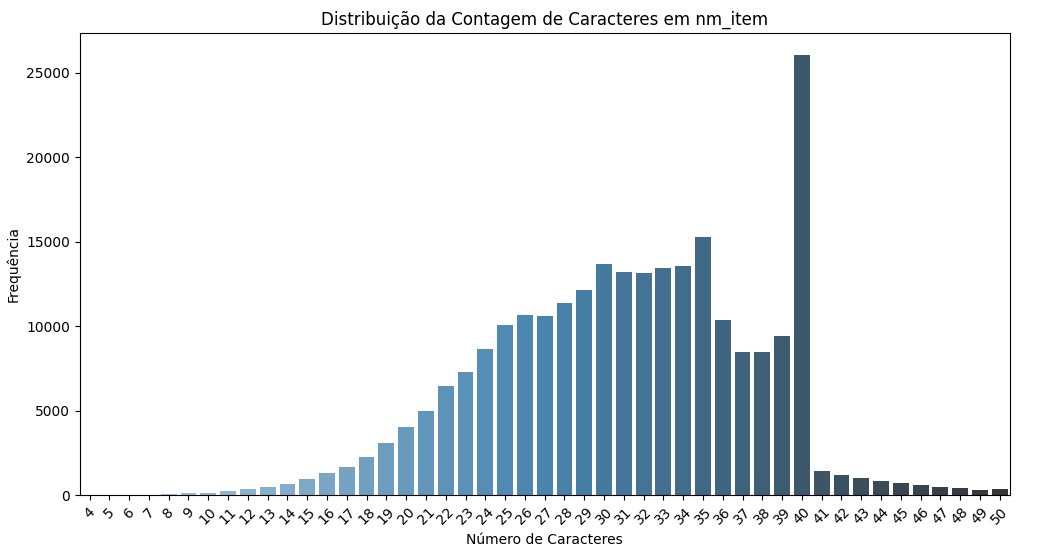
\includegraphics[width=0.8\textwidth]{images/distcaracteres.png}
    \caption{Distribuição de frequencia da contagem de caracteres por descrição.}
    \label{fig:distcaracteres}
\end{figure}

\subsubsection{Distribuição de Palavras por Descrição}
A Figura \ref{fig:distpalavras} apresenta a distribuição por palavra. Esta mostra uma predominância de descrições com 4 a 6 palavras, refletindo uma tendência à concisão nas descrições dos produtos. Este padrão é indicativo de um esforço para comunicar informações essenciais de forma eficiente, permitindo aos consumidores entender rapidamente as características dos produtos.

\begin{figure}[H]
    \centering
    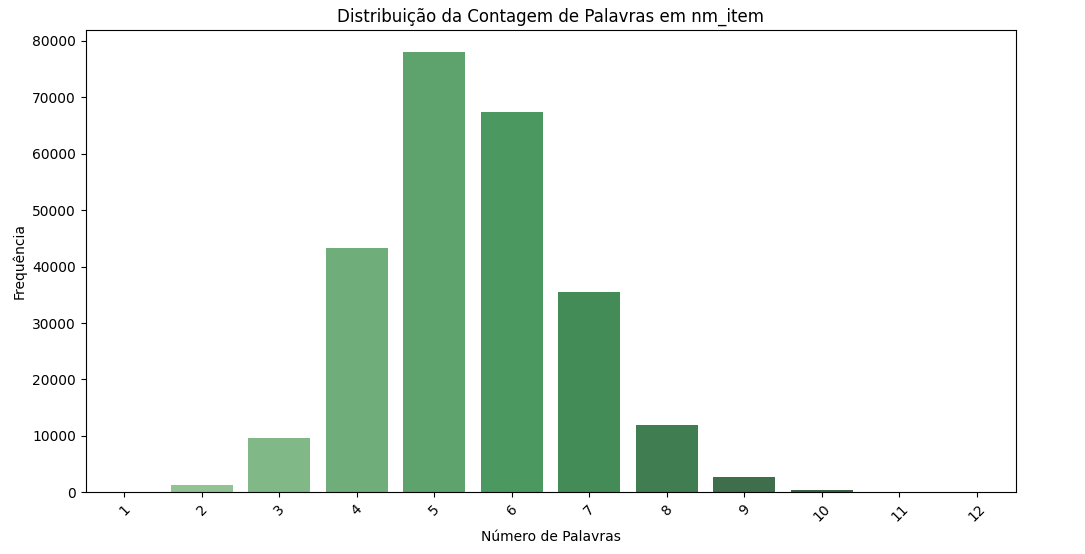
\includegraphics[width=0.8\textwidth]{images/distpalavrass.png}
    \caption{Distribuição de frequencia da contagem de palavras por descrição.}
    \label{fig:distpalavras}
\end{figure}

\subsection{Pré-Processamento}

Conforme discutido na seção \ref{subsec:preprocessamento}, a normalização, incluindo a remoção de acentos e a conversão para letras minúsculas, é adotada para uniformizar as variações linguísticas. Esta abordagem facilita a análise dos dados, alinhando-se com as práticas padrão em processamento de linguagem natural.  Diversas técnicas são apresentadas, mas as de maior impacto são a \textbf{normalização e conversão para minúsculas}.  As demais, conforme \cite{naseem2021survey}, acabam não impactando significativamente no resultado final.  Cabe ressaltar que as descrições de produto não apresentam verbos e variantes com prefixo e sufixo.

\subsection{Tokenização}
A tokenização é realizada para decompor os textos em unidades menores, ou tokens. Neste trabalho, serão exploradas representações baseadas em unigramas, bigramas e seqgramas. Esta decisão é fundamentada pela necessidade de capturar tanto a frequência de palavras individuais (\textit{unigramas}) quanto as relações entre palavras adjacentes (\textit{bigramas}) e sequências de palavras (\textit{seqgramas}), conforme destacado na seção \ref{subsec:tokenizacao}.

\subsection{Vetorização}
Utilizam-se as técnicas de Bag of Words (BoW), Term Frequency (TF), e Term Frequency-Inverse Document Frequency (TFIDF) para transformar os textos tokenizados em representações vetoriais. Estas técnicas são aplicadas a unigramas, bigramas e seqgramas, tanto em formas normalizadas quanto não-normalizadas, para capturar a importância relativa das palavras e suas relações contextuais.  Estas técnicas são descritas na seção \ref{subsec:representacaonumerica} sobre representação numérica.  A escolha se deve a ser os principais modelos utilizados pelas literaturas.

São avaliadas as representações vetoriais em suas formas normalizadas e não-normalizadas. A normalização dos vetores de características visa a padronização à uma escala comum, facilitando a integração de diferentes tipos de características e a aplicação de algoritmos de aprendizado de máquina.

\subsection{Seleção de Modelos}

Com base nos fundamentos apresentados anteriormente, a seleção de modelos para este estudo foi conduzida considerando-se as características distintas da classificação de textos curtos. Identificou-se que a natureza concisa dos dados demanda métodos capazes de extrair eficientemente a informação semântica limitada. Portanto, optou-se por avaliar tanto métodos de recuperação de informação, com ênfase no método baseado em similaridade, quanto modelos tradicionais de aprendizado de máquina, incluindo Naive Bayes (NB), Árvores de Decisão (DT), Máquinas de Vetores de Suporte (SVM), k-Nearest Neighbors (KNN) e Regressão Logística (RL).

\subsubsection{Argmax da Similaridade}

A adoção de métodos baseados em argmax para a classificação de texto neste estudo é justificada pela necessidade de um procedimento fundamentada na similaridade do conteúdo. Esses métodos servem como pontos iniciais para análises mais aprofundadas, proporcionando uma eficiente categorização preliminar de documentos. Além disso, a simplicidade desses métodos auxilia na interpretação dos resultados e na comparação com abordagens mais complexas, estabelecendo uma base sólida para a exploração de métodos adicionais.

\paragraph{Vantagens e Desvantagens}
\textbf{Vantagens:}
\begin{itemize}
    \item Simplicidade de Implementação: Facilita a compreensão e a implementação.
    \item Eficiência Computacional: Permite execução rápida, especialmente em conjuntos de dados volumosos.
    \item Adaptabilidade: Aplica-se a diferentes métricas de similaridade.
\end{itemize}

\textbf{Desvantagens:}
\begin{itemize}
    \item Sensibilidade a Distorções nos Dados: Vulnerabilidade a ruídos e outliers.
    \item Desconsideração da Distribuição de Similaridade: Foco exclusivo no valor máximo, ignorando a distribuição global de similaridades.
    \item Limitação em Contextos Complexos: Dificuldade em capturar nuances em textos com múltiplas interpretações ou categorias próximas.
\end{itemize}

\subsubsection{Modelos Tradicionais}
\begin{itemize}
    \item \textbf{Naive Bayes (NB):} Selecionado pela sua eficiência e simplicidade, reconhecido por sua robustez na classificação de texto.
    
    \item \textbf{Árvores de Decisão (DT):} Escolhidas pela capacidade de abordar características não lineares e pela facilidade de interpretação dos modelos gerados.
    
    \item \textbf{Máquinas de Vetores de Suporte (SVM):} A eficácia em espaços de alta dimensão motivou sua seleção.
    
    \item \textbf{k-Nearest Neighbors (KNN):} A simplicidade e eficácia em classificações que não demandam modelos complexos foram as principais razões para sua escolha.
    
    \item \textbf{Regressão Logística (RL):} Incluída por sua habilidade em fornecer probabilidades de classe, útil para classificar descrições ambíguas.
\end{itemize}

\paragraph{Considerações}
A exclusão de modelos de aprendizado profundo, técnicas de bagging e boosting, bem como modelos baseados em word embeddings, foi uma decisão intencional, motivada pela limitação de escopo deste trabalho. Esta pesquisa estabelece uma fundação inicial, focando em métodos tradicionais e de recuperação de informação, pavimentando o caminho para futuros estudos que possam explorar métodos mais avançados e contemporâneos. A diversidade dos modelos selecionados permite uma avaliação abrangente das técnicas de classificação de texto, maximizando as chances de identificar o método mais eficaz para o conjunto de dados específico.

\subsection{Métricas de Avaliação}

O principal objetivo das métricas de avaliação é fornecer um quadro confiável para a análise do desempenho dos modelos. Procurou-se selecionar métricas que considerassem tanto a eficácia geral do modelo quanto sua capacidade de tratar classes de maneira equitativa, evitando viés em favor das classes mais representativas no conjunto de dados.  Desta forma, pode-se resumir o objetivo em \textit{abrangência} e \textit{equidade}.  Segundo Tharwat (2018) e Grandini et al. (2020), as métricas são fundamentais para compreender o desempenho dos modelos em contextos multiclasse, onde a complexidade e o desbalanceamento entre classes apresentam desafios significativos.
Para satisfazer estes dois critérios foram escolhidas a \textbf{F1-Score Macro} e \textbf{Acurácia}. Elas juntas proporcionam uma visão equilibrada e abrangente do desempenho dos modelos.
Quanto a \textbf{abrangência} a acurácia fornece uma visão geral do desempenho enquanto que para a \textbf{equidade} A F1-score macro, ao calcular a média dos F1-Scores de todas as classes, dá igual peso a cada uma delas, favorecendo uma avaliação justa independentemente do tamanho da classe.

\subsection{Configurações de Treinamento}

Para avaliar o desempenho dos modelos de aprendizado de máquina especificados neste estudo, o conjunto de dados foi submetido a um processo de randomização antes da aplicação das técnicas de treinamento. A técnica de validação cruzada k-fold com 10 partições foi adotada, baseando-se na recomendação de \cite{kohavi1995study}, que destaca a eficiência desta abordagem em proporcionar estimativas confiáveis do desempenho dos modelos.

O procedimento foi realizado da seguinte forma: após a randomização do conjunto de dados, este foi dividido em 10 partições de tamanho igual. Utilizando a abordagem de validação cruzada, em cada ciclo, nove partições foram empregadas para o treinamento do modelo, enquanto a partição restante foi reservada para teste. Este processo foi repetido 10 vezes, com cada partição servindo exatamente uma vez como conjunto de teste. Essa metodologia assegura uma avaliação completa e equitativa do desempenho dos modelos avaliados no trabalho.

\subsection{Ajuste Fino dos Modelos}

O ajuste fino dos hiperparâmetros visa otimizar o desempenho dos modelos de aprendizado de máquina. Nesta seção, é descrito os hiperparâmetros que serão avaliados para cada modelo utilizado neste estudo.

\subsubsection{Métodos Baseados em Argmax}

Para os métodos baseados em argmax, as combinações dos seguintes hiperparâmetros serão avaliadas:

\begin{itemize}
    \item \textbf{Tokenização}: Serão exploradas três abordagens distintas para a tokenização: unigramas, bigramas e seqgramas. Essas abordagens permitem analisar a influência do tamanho dos tokens na performance do modelo.
    \item \textbf{Vetorização}: É avaliada três técnicas de vetorização: binária, frequência e TF-IDF (Term Frequency-Inverse Document Frequency). Cada técnica fornece uma representação diferente dos textos, que será examinada em termos de impacto no desempenho do modelo.
    \item \textbf{Normalização}: Será considerada a aplicação ou não de normalização nos textos, incluindo a conversão para minúsculas e remoção de acentos, para verificar sua influência na eficácia do modelo.
\end{itemize}

A combinação desses hiperparâmetros visa explorar uma ampla gama de configurações para identificar aquela que proporciona o melhor desempenho para a classificação de texto baseada em argmax. A tabela \ref{tab:combinacoes} exibe as combinações avaliadas.

\begin{table}[H]
\centering
\caption{Combinações de Tokenização, Vetorização e Normalização}
\label{tab:combinacoes}
\begin{tabular}{l|l|l|l}
\hline
\textbf{ID} & \textbf{Tokenização} & \textbf{Tipo} & \textbf{Normalização} \\ \hline
ARGMAX1BI            & unigram     & Binário &               \\ \hline
ARGMAX1BINORM        & unigram     & Binário & Normalizado   \\ \hline
ARGMAX1TF            & unigram     & TF      &               \\ \hline
ARGMAX1TFNORM        & unigram     & TF      & Normalizado   \\ \hline
ARGMAX1TFIDF         & unigram     & TFIDF   &               \\ \hline
ARGMAX1TFIDFNORM     & unigram     & TFIDF   & Normalizado   \\ \hline
ARGMAX2BI            & bigram      & Binário &               \\ \hline
ARGMAX2BINORM        & bigram      & Binário & Normalizado   \\ \hline
ARGMAX2TF            & bigram      & TF      &               \\ \hline
ARGMAX2TFNORM        & bigram      & TF      & Normalizado   \\ \hline
ARGMAX2TFIDF         & bigram      & TFIDF   &               \\ \hline
ARGMAX2TFIDFNORM     & bigram      & TFIDF   & Normalizado   \\ \hline
ARGMAXSBI            & seqgram     & Binário &               \\ \hline
ARGMAXSBINORM        & seqgram     & Binário & Normalizado   \\ \hline
ARGMAXSTF            & seqgram     & TF      &               \\ \hline
ARGMAXSTFNORM        & seqgram     & TF      & Normalizado   \\ \hline
ARGMAXSTFIDF         & seqgram     & TFIDF   &               \\ \hline
ARGMAXSTFIDFNORM     & seqgram     & TFIDF   & Normalizado   \\ \hline
\end{tabular}
\end{table}

\subsubsection{Modelos de Aprendizado de Máquina}

O processo de ajuste fino para os modelos de aprendizado de máquina específicos será detalhado a seguir, focando nos hiperparâmetros chave de cada um:

\paragraph{Máquina de Vetores de Suporte (SVM)}

A Máquina de Vetores de Suporte (SVM) é um modelo de aprendizado de máquina baseado em otimização, projetado para encontrar um hiperplano que minimize a distância até os vetores mais próximos de classes distintas, conhecidos como vetores de suporte. A formulação matemática do SVM é expressa pela seguinte equação, adaptada de \cite{pedregosa2011scikit}:

\begin{equation}
\label{eq6}
\begin{aligned}\min_ {w, b, \zeta} \frac{1}{2} w^T w + C \sum_{i=1}^{n} \zeta_i\\
\begin{split}\textrm {sujeito a} \\
& y_i (w^T \phi (x_i) + b) \geq 1 - \zeta_i,\\
& \zeta_i \geq 0, i=1, ..., n\end{split}
\end{aligned}
\end{equation}

Durante o processo de ajuste fino, os seguintes hiperparâmetros do SVM serão avaliados:

\begin{itemize}
    \item \textbf{Funções de Kernel:} Diferentes funções de kernel, incluindo linear, polinomial, radial (RBF) e sigmoide, serão testadas. O kernel transforma o espaço de entrada em um espaço de maior dimensão onde é possível encontrar um hiperplano de separação linear.
    \item \textbf{C (Parâmetro de Regularização):} O parâmetro C, que controla o trade-off entre a maximização da margem e a minimização do erro de classificação, será ajustado. Valores mais altos de C indicam uma menor tolerância a erros de classificação.
    \item \textbf{Peso da Classe:} Este hiperparâmetro ajusta o peso das classes, sendo particularmente útil em situações de desbalanceamento de classes.
    \item \textbf{Grau (para Kernel Polinomial):} Quando o kernel polinomial é selecionado, o grau do polinômio representa um hiperparâmetro crítico que será ajustado.
\end{itemize}

A seleção e o ajuste desses hiperparâmetros serão realizados por meio de técnicas como busca em grade (Grid Search) ou busca aleatória (Random Search), com o objetivo de identificar a configuração que maximiza a precisão do modelo SVM no conjunto de dados utilizado neste estudo.

\paragraph{Regressão Logística}

A Regressão Logística (RL) é empregada como um modelo de classificação no contexto de aprendizado de máquina supervisionado. A formulação matemática da RL, adaptada de \cite{pedregosa2011scikit}, é apresentada abaixo:

\begin{equation}
\label{eq5}
\min_{w, c} \frac{1 - \rho}{2}w^T w + \rho \|w\|_1 + \\ C \sum_{i=1}^n \\ \log\left (e^{-y_i (X_i^T w + c)} + 1\right )
\end{equation}

Durante o ajuste fino, os seguintes hiperparâmetros da Regressão Logística serão explorados:

\begin{itemize}
    \item \textbf{Solver:} O método de otimização a ser utilizado na minimização da função de custo. O solver "saga" foi escolhido por sua eficiência em conjuntos de dados de grande escala.
    \item \textbf{Penalidade (Penalty):} Representa o tipo de regularização aplicada ao modelo. Serão testadas as opções "l1" (norma L1), "l2" (norma L2) e "elasticnet", que é uma combinação linear das penalidades L1 e L2. A relevância de cada tipo de penalidade será determinada pelo ajuste do hiperparâmetro \(\rho\) (l1\_ratio) no caso de "elasticnet".
    \item \textbf{C (Parâmetro de Regularização):} Controla a força da regularização inversamente. Valores mais altos de C correspondem a uma regularização menos rigorosa. Serão avaliados diferentes valores de C para identificar o equilíbrio ideal entre bias e variância.
    \item \textbf{Peso da Classe (Class Weight):} Este hiperparâmetro ajusta os pesos das classes no cálculo da função de custo, sendo particularmente útil em situações com classes desbalanceadas. A opção "balanceada" será comparada ao cenário onde todas as classes têm o mesmo peso.
\end{itemize}

O processo de ajuste desses hiperparâmetros visa otimizar o desempenho da Regressão Logística no conjunto de dados estudado, utilizando técnicas como busca em grade (Grid Search) para explorar o espaço de hiperparâmetros de forma sistemática.

\paragraph{Árvores de Decisão}

As Árvores de Decisão são modelos de aprendizado de máquina supervisionado amplamente utilizados para tarefas de classificação e regressão. Esses modelos são preferidos por sua facilidade de interpretação, a capacidade de lidar com dados não lineares e a não necessidade de normalização dos dados. A formulação matemática específica para uma árvore de decisão é mais intuitiva, focando na divisão do espaço de dados em regiões homogêneas com base nos valores dos atributos.

Durante o processo de ajuste fino, os seguintes hiperparâmetros das Árvores de Decisão serão avaliados:

\begin{itemize}
    \item \textbf{Critério:} O critério utilizado para medir a qualidade de uma divisão. Os critérios mais comuns são "gini" para a impureza de Gini e "entropy" para o ganho de informação (entropia), sendo ambos avaliados para determinar qual oferece o melhor desempenho para o modelo.
    \item \textbf{Profundidade Máxima da Árvore (max\_depth):} A profundidade máxima da árvore será ajustada para controlar a complexidade do modelo, prevenindo overfitting. Serão testados valores variados para encontrar o equilíbrio ideal entre bias e variância.
    \item \textbf{Número Mínimo de Amostras para Dividir um Nó (min\_samples\_split):} Este hiperparâmetro determina o número mínimo de amostras necessárias para dividir um nó interno. Valores diferentes serão explorados para otimizar a capacidade da árvore de generalizar bem para dados não vistos.
    \item \textbf{Número Mínimo de Amostras em um Nó Folha (min\_samples\_leaf):} O número mínimo de amostras requeridas para estar em um nó folha. Ajustar esse parâmetro ajuda a suavizar o modelo, especialmente em casos de dados ruidosos.
\end{itemize}

O ajuste desses hiperparâmetros será realizado por meio de técnicas de busca, como a busca em grade (Grid Search) ou busca aleatória (Random Search), com o objetivo de identificar a configuração que maximiza a precisão da árvore de decisão no conjunto de dados utilizado neste estudo.

\paragraph{k-Nearest Neighbors (KNN)}

O k-Nearest Neighbors (KNN) é um algoritmo simples, porém poderoso, utilizado tanto para classificação quanto para regressão. Baseia-se no princípio de que as amostras mais próximas no espaço de características tendem a pertencer à mesma classe. O KNN é particularmente apreciado por sua facilidade de implementação e sua eficácia em uma ampla gama de problemas.

Durante o processo de ajuste fino, os seguintes hiperparâmetros do KNN serão avaliados:

\begin{itemize}
    \item \textbf{Número de Vizinhos (n\_neighbors):} O número de vizinhos a considerar determina a fronteira de decisão do KNN. Serão testados diferentes valores para encontrar o número ótimo de vizinhos que maximiza a precisão do modelo.
    \item \textbf{Peso dos Vizinhos (weights):} O peso atribuído aos vizinhos pode ser uniforme, onde todos os vizinhos contribuem igualmente, ou baseado na distância, onde vizinhos mais próximos têm uma influência maior na decisão. Ambas as opções serão exploradas para determinar qual oferece o melhor desempenho.
    \item \textbf{Métrica de Distância (metric):} A escolha da métrica de distância (como distância euclidiana, manhattan, minkowski, ou hamming) é crucial para o desempenho do KNN. Diferentes métricas serão avaliadas para identificar a mais adequada para o conjunto de dados em questão.
    \item \textbf{Algoritmo para Computação da Distância (algorithm):} As opções incluem 'ball\_tree', 'kd\_tree', 'brute', e 'auto', influenciando a eficiência do cálculo das distâncias. O algoritmo mais eficiente para o nosso conjunto de dados será identificado mediante experimentação.
\end{itemize}

O processo de ajuste desses hiperparâmetros será conduzido utilizando técnicas como a busca em grade (Grid Search) ou busca aleatória (Random Search), visando encontrar a configuração que oferece o melhor equilíbrio entre precisão e eficiência computacional para o modelo KNN no conjunto de dados utilizado neste estudo.

\paragraph{Naive Bayes}

O Naive Bayes é um classificador probabilístico baseado no teorema de Bayes, com a "ingênua" suposição de independência entre os preditores. Apesar de sua simplicidade, o Naive Bayes pode ser surpreendentemente eficaz e é frequentemente utilizado em tarefas de classificação de texto e filtragem de spam.

No ajuste fino do modelo Naive Bayes, focaremos na seleção do tipo de modelo Naive Bayes apropriado para o nosso conjunto de dados, uma vez que diferentes variantes são mais adequadas para diferentes tipos de distribuição de dados. Os seguintes hiperparâmetros e variantes do modelo serão avaliados:

\begin{itemize}
    \item \textbf{Tipo de Modelo Naive Bayes:} Dependendo da natureza do conjunto de dados, diferentes versões do Naive Bayes serão testadas, incluindo:
    \begin{itemize}
        \item Gaussian Naive Bayes: Ideal para características com distribuição normal.
        \item Multinomial Naive Bayes: Adequado para dados distribuídos multinomialmente, como a contagem de palavras em textos.
        \item Bernoulli Naive Bayes: Utilizado para características binárias/multivariáveis.
        \item Complement Naive Bayes: Uma adaptação do Multinomial Naive Bayes que é particularmente adequada para conjuntos de dados desbalanceados.
    \end{itemize}
    \item \textbf{Suavização Laplaciana (alpha):} Para modelos como Multinomial e Bernoulli Naive Bayes, a suavização Laplaciana (ou aditiva) é aplicada para lidar com o problema de probabilidade zero. O valor de $\alpha$ será ajustado para otimizar o desempenho do modelo.
\end{itemize}

A seleção do modelo e o ajuste do hiperparâmetro de suavização serão realizados por meio de validação cruzada, com o objetivo de identificar a configuração que oferece a melhor acurácia para a classificação no conjunto de dados estudado.


